\documentclass[twoside]{book}

% Packages required by doxygen
\usepackage{fixltx2e}
\usepackage{calc}
\usepackage{doxygen}
\usepackage[export]{adjustbox} % also loads graphicx
\usepackage{graphicx}
\usepackage[utf8]{inputenc}
\usepackage{makeidx}
\usepackage{multicol}
\usepackage{multirow}
\PassOptionsToPackage{warn}{textcomp}
\usepackage{textcomp}
\usepackage[nointegrals]{wasysym}
\usepackage[table]{xcolor}

% NLS support packages
\usepackage[brazil]{babel}
% Font selection
\usepackage[T1]{fontenc}
\usepackage[scaled=.90]{helvet}
\usepackage{courier}
\usepackage{amssymb}
\usepackage{sectsty}
\renewcommand{\familydefault}{\sfdefault}
\allsectionsfont{%
  \fontseries{bc}\selectfont%
  \color{darkgray}%
}
\renewcommand{\DoxyLabelFont}{%
  \fontseries{bc}\selectfont%
  \color{darkgray}%
}
\newcommand{\+}{\discretionary{\mbox{\scriptsize$\hookleftarrow$}}{}{}}

% Page & text layout
\usepackage{geometry}
\geometry{%
  a4paper,%
  top=2.5cm,%
  bottom=2.5cm,%
  left=2.5cm,%
  right=2.5cm%
}
\tolerance=750
\hfuzz=15pt
\hbadness=750
\setlength{\emergencystretch}{15pt}
\setlength{\parindent}{0cm}
\setlength{\parskip}{3ex plus 2ex minus 2ex}
\makeatletter
\renewcommand{\paragraph}{%
  \@startsection{paragraph}{4}{0ex}{-1.0ex}{1.0ex}{%
    \normalfont\normalsize\bfseries\SS@parafont%
  }%
}
\renewcommand{\subparagraph}{%
  \@startsection{subparagraph}{5}{0ex}{-1.0ex}{1.0ex}{%
    \normalfont\normalsize\bfseries\SS@subparafont%
  }%
}
\makeatother

% Headers & footers
\usepackage{fancyhdr}
\pagestyle{fancyplain}
\fancyhead[LE]{\fancyplain{}{\bfseries\thepage}}
\fancyhead[CE]{\fancyplain{}{}}
\fancyhead[RE]{\fancyplain{}{\bfseries\leftmark}}
\fancyhead[LO]{\fancyplain{}{\bfseries\rightmark}}
\fancyhead[CO]{\fancyplain{}{}}
\fancyhead[RO]{\fancyplain{}{\bfseries\thepage}}
\fancyfoot[LE]{\fancyplain{}{}}
\fancyfoot[CE]{\fancyplain{}{}}
\fancyfoot[RE]{\fancyplain{}{\bfseries\scriptsize Gerado por Doxygen }}
\fancyfoot[LO]{\fancyplain{}{\bfseries\scriptsize Gerado por Doxygen }}
\fancyfoot[CO]{\fancyplain{}{}}
\fancyfoot[RO]{\fancyplain{}{}}
\renewcommand{\footrulewidth}{0.4pt}
\renewcommand{\chaptermark}[1]{%
  \markboth{#1}{}%
}
\renewcommand{\sectionmark}[1]{%
  \markright{\thesection\ #1}%
}

% Indices & bibliography
\usepackage{natbib}
\usepackage[titles]{tocloft}
\setcounter{tocdepth}{3}
\setcounter{secnumdepth}{5}
\makeindex

% Hyperlinks (required, but should be loaded last)
\usepackage{ifpdf}
\ifpdf
  \usepackage[pdftex,pagebackref=true]{hyperref}
\else
  \usepackage[ps2pdf,pagebackref=true]{hyperref}
\fi
\hypersetup{%
  colorlinks=true,%
  linkcolor=blue,%
  citecolor=blue,%
  unicode%
}

% Custom commands
\newcommand{\clearemptydoublepage}{%
  \newpage{\pagestyle{empty}\cleardoublepage}%
}

\usepackage{caption}
\captionsetup{labelsep=space,justification=centering,font={bf},singlelinecheck=off,skip=4pt,position=top}

%===== C O N T E N T S =====

\begin{document}

% Titlepage & ToC
\hypersetup{pageanchor=false,
             bookmarksnumbered=true,
             pdfencoding=unicode
            }
\pagenumbering{alph}
\begin{titlepage}
\vspace*{7cm}
\begin{center}%
{\Large Similador de mémoria cache }\\
\vspace*{1cm}
{\large Gerado por Doxygen 1.8.13}\\
\end{center}
\end{titlepage}
\clearemptydoublepage
\pagenumbering{roman}
\tableofcontents
\clearemptydoublepage
\pagenumbering{arabic}
\hypersetup{pageanchor=true}

%--- Begin generated contents ---
\chapter{Índice Hierárquico}
\section{Hierarquia de Classes}
Esta lista de hierarquias está parcialmente ordenada (ordem alfabética)\+:\begin{DoxyCompactList}
\item \contentsline{section}{App}{\pageref{classApp}}{}
\item \contentsline{section}{Bloco}{\pageref{structBloco}}{}
\begin{DoxyCompactList}
\item \contentsline{section}{Linha}{\pageref{structLinha}}{}
\end{DoxyCompactList}
\item \contentsline{section}{Cache}{\pageref{structCache}}{}
\item \contentsline{section}{Config}{\pageref{structConfig}}{}
\item \contentsline{section}{Memoria}{\pageref{structMemoria}}{}
\item \contentsline{section}{Random}{\pageref{structRandom}}{}
\end{DoxyCompactList}

\chapter{Índice dos Componentes}
\section{Lista de Componentes}
Aqui estão as classes, estruturas, uniões e interfaces e suas respectivas descrições\+:\begin{DoxyCompactList}
\item\contentsline{section}{\hyperlink{classApp}{App} \\*Classe responsável tanto pelo front-\/end quanto pelo back-\/end da aplicação. Essa decisão foi tomada para deixar o código mais simples }{\pageref{classApp}}{}
\item\contentsline{section}{\hyperlink{structBloco}{Bloco} \\*A classe bloco representa um endereço da mémoria que armazena \{numero\+\_\+de\+\_\+palavras\} palavras }{\pageref{structBloco}}{}
\item\contentsline{section}{\hyperlink{structCache}{Cache} \\*A cache é uma mémoria próxima do processador }{\pageref{structCache}}{}
\item\contentsline{section}{\hyperlink{structConfig}{Config} \\*Estrutura que armazena as variaveis com a configuração }{\pageref{structConfig}}{}
\item\contentsline{section}{\hyperlink{structLinha}{Linha} \\*A linha é um bloco da cache, com a diferença que ela contém os contadores }{\pageref{structLinha}}{}
\item\contentsline{section}{\hyperlink{structMemoria}{Memoria} \\*A mémoria é um conjunto de blocos }{\pageref{structMemoria}}{}
\item\contentsline{section}{\hyperlink{structRandom}{Random} \\*Functor (objeto de função) para gerar números aléatorios não negativos de três digitos }{\pageref{structRandom}}{}
\end{DoxyCompactList}

\chapter{Classes}
\hypertarget{classApp}{}\section{Referência da Classe App}
\label{classApp}\index{App@{App}}


Classe responsável tanto pelo front-\/end quanto pelo back-\/end da aplicação. Essa decisão foi tomada para deixar o código mais simples.  




{\ttfamily \#include $<$app.\+hpp$>$}

\subsection*{Métodos Públicos}
\begin{DoxyCompactItemize}
\item 
\hyperlink{classApp_a9035c72be7a12b46180e6d45b87436ee}{App} (\hyperlink{structConfig}{Config} cfg)
\begin{DoxyCompactList}\small\item\em Construtor da classe \hyperlink{classApp}{App}. \end{DoxyCompactList}\item 
void \hyperlink{classApp_ade8467361fe8300a45ee03433a5da7be}{read} (unsigned int endereco)
\begin{DoxyCompactList}\small\item\em Ler um bloco da mémoria (trazer para uma linha da cache). \end{DoxyCompactList}\item 
void \hyperlink{classApp_ab72f344e7a9f4113c8624bdb2cfd16ee}{write} (unsigned int endereco, unsigned int valor)
\begin{DoxyCompactList}\small\item\em Escreve em um endereço de mémoria um valor. \end{DoxyCompactList}\item 
\mbox{\Hypertarget{classApp_aa4c457ebcb748c398fa044140514188c}\label{classApp_aa4c457ebcb748c398fa044140514188c}} 
void \hyperlink{classApp_aa4c457ebcb748c398fa044140514188c}{show} ()
\begin{DoxyCompactList}\small\item\em Exibe o mapa de mémoria atual da cache e da mémoria. \end{DoxyCompactList}\end{DoxyCompactItemize}


\subsection{Descrição Detalhada}
Classe responsável tanto pelo front-\/end quanto pelo back-\/end da aplicação. Essa decisão foi tomada para deixar o código mais simples. 

\subsection{Construtores \& Destrutores}
\mbox{\Hypertarget{classApp_a9035c72be7a12b46180e6d45b87436ee}\label{classApp_a9035c72be7a12b46180e6d45b87436ee}} 
\index{App@{App}!App@{App}}
\index{App@{App}!App@{App}}
\subsubsection{\texorpdfstring{App()}{App()}}
{\footnotesize\ttfamily App\+::\+App (\begin{DoxyParamCaption}\item[{\hyperlink{structConfig}{Config}}]{cfg }\end{DoxyParamCaption})}



Construtor da classe \hyperlink{classApp}{App}. 


\begin{DoxyParams}{Parâmetros}
{\em cfg} & Configuração já lida. \\
\hline
\end{DoxyParams}


\subsection{Métodos}
\mbox{\Hypertarget{classApp_ade8467361fe8300a45ee03433a5da7be}\label{classApp_ade8467361fe8300a45ee03433a5da7be}} 
\index{App@{App}!read@{read}}
\index{read@{read}!App@{App}}
\subsubsection{\texorpdfstring{read()}{read()}}
{\footnotesize\ttfamily void App\+::read (\begin{DoxyParamCaption}\item[{unsigned int}]{endereco }\end{DoxyParamCaption})}



Ler um bloco da mémoria (trazer para uma linha da cache). 


\begin{DoxyParams}{Parâmetros}
{\em endereco} & \\
\hline
\end{DoxyParams}
\mbox{\Hypertarget{classApp_ab72f344e7a9f4113c8624bdb2cfd16ee}\label{classApp_ab72f344e7a9f4113c8624bdb2cfd16ee}} 
\index{App@{App}!write@{write}}
\index{write@{write}!App@{App}}
\subsubsection{\texorpdfstring{write()}{write()}}
{\footnotesize\ttfamily void App\+::write (\begin{DoxyParamCaption}\item[{unsigned int}]{endereco,  }\item[{unsigned int}]{valor }\end{DoxyParamCaption})}



Escreve em um endereço de mémoria um valor. 

\begin{DoxyNote}{Observação}
O endereço não precisa necessáriamente estar na cache, pois será feito o mapeamento. 

Faz o Write Though se definido nas configurações. 
\end{DoxyNote}

\begin{DoxyParams}{Parâmetros}
{\em endereco} & Endereco de escrita. \\
\hline
{\em valor} & Valor a ser escrita. \\
\hline
\end{DoxyParams}


A documentação para esta classe foi gerada a partir do seguinte arquivo\+:\begin{DoxyCompactItemize}
\item 
include/app.\+hpp\end{DoxyCompactItemize}

\hypertarget{structBloco}{}\section{Referência da Estrutura Bloco}
\label{structBloco}\index{Bloco@{Bloco}}


A classe bloco representa um endereço da mémoria que armazena \{numero\+\_\+de\+\_\+palavras\} palavras.  




{\ttfamily \#include $<$cache.\+hpp$>$}



Diagrama de Hierarquia para Bloco\+:\nopagebreak
\begin{figure}[H]
\begin{center}
\leavevmode
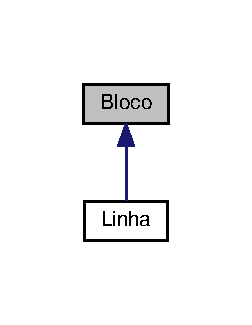
\includegraphics[width=121pt]{structBloco__inherit__graph}
\end{center}
\end{figure}
\subsection*{Métodos Públicos}
\begin{DoxyCompactItemize}
\item 
\hyperlink{structBloco_a7690a145e0f647595d28c633d034abb3}{Bloco} (unsigned int tamanho)
\begin{DoxyCompactList}\small\item\em Cria um bloco de \{tamanho\} palavras. \end{DoxyCompactList}\item 
\hyperlink{structBloco_a23af86d8bfc57541015b41571d4558f8}{Bloco} (unsigned int tamanho, \hyperlink{structRandom}{Random} \&rand)
\begin{DoxyCompactList}\small\item\em Criar um bloco de \{tamanho\} palavras com conteúdo aleatório. \end{DoxyCompactList}\end{DoxyCompactItemize}
\subsection*{Atributos Públicos}
\begin{DoxyCompactItemize}
\item 
\mbox{\Hypertarget{structBloco_ac6dbb14d476c08f86f91bcb6fbce4e20}\label{structBloco_ac6dbb14d476c08f86f91bcb6fbce4e20}} 
std\+::vector$<$ unsigned int $>$ \hyperlink{structBloco_ac6dbb14d476c08f86f91bcb6fbce4e20}{conteudo}
\begin{DoxyCompactList}\small\item\em Palavras contidas no bloco. \end{DoxyCompactList}\end{DoxyCompactItemize}


\subsection{Descrição Detalhada}
A classe bloco representa um endereço da mémoria que armazena \{numero\+\_\+de\+\_\+palavras\} palavras. 

\subsection{Construtores \& Destrutores}
\mbox{\Hypertarget{structBloco_a7690a145e0f647595d28c633d034abb3}\label{structBloco_a7690a145e0f647595d28c633d034abb3}} 
\index{Bloco@{Bloco}!Bloco@{Bloco}}
\index{Bloco@{Bloco}!Bloco@{Bloco}}
\subsubsection{\texorpdfstring{Bloco()}{Bloco()}\hspace{0.1cm}{\footnotesize\ttfamily [1/2]}}
{\footnotesize\ttfamily Bloco\+::\+Bloco (\begin{DoxyParamCaption}\item[{unsigned int}]{tamanho }\end{DoxyParamCaption})\hspace{0.3cm}{\ttfamily [inline]}}



Cria um bloco de \{tamanho\} palavras. 


\begin{DoxyParams}{Parâmetros}
{\em tamanho} & quantidade de palavras. \\
\hline
\end{DoxyParams}
\mbox{\Hypertarget{structBloco_a23af86d8bfc57541015b41571d4558f8}\label{structBloco_a23af86d8bfc57541015b41571d4558f8}} 
\index{Bloco@{Bloco}!Bloco@{Bloco}}
\index{Bloco@{Bloco}!Bloco@{Bloco}}
\subsubsection{\texorpdfstring{Bloco()}{Bloco()}\hspace{0.1cm}{\footnotesize\ttfamily [2/2]}}
{\footnotesize\ttfamily Bloco\+::\+Bloco (\begin{DoxyParamCaption}\item[{unsigned int}]{tamanho,  }\item[{\hyperlink{structRandom}{Random} \&}]{rand }\end{DoxyParamCaption})\hspace{0.3cm}{\ttfamily [inline]}}



Criar um bloco de \{tamanho\} palavras com conteúdo aleatório. 


\begin{DoxyParams}{Parâmetros}
{\em tamanho} & quantidade de palavras. \\
\hline
{\em rand} & Functor de geração de números ramdomicos. \\
\hline
\end{DoxyParams}


A documentação para esta estrutura foi gerada a partir do seguinte arquivo\+:\begin{DoxyCompactItemize}
\item 
include/cache.\+hpp\end{DoxyCompactItemize}

\hypertarget{structCache}{}\section{Referência da Estrutura Cache}
\label{structCache}\index{Cache@{Cache}}


A cache é uma mémoria próxima do processador.  




{\ttfamily \#include $<$cache.\+hpp$>$}

\subsection*{Métodos Públicos}
\begin{DoxyCompactItemize}
\item 
\hyperlink{structCache_a9f868538691619d64b59b858ae0461a8}{Cache} (unsigned int tamanho, unsigned int numero\+\_\+de\+\_\+palavras)
\begin{DoxyCompactList}\small\item\em Constrói uma memoria cache de \{tamanho\} linha(blocos) com cada bloco contendo \{numero\+\_\+de\+\_\+palavras\} palavras. \end{DoxyCompactList}\end{DoxyCompactItemize}
\subsection*{Atributos Públicos}
\begin{DoxyCompactItemize}
\item 
\mbox{\Hypertarget{structCache_ad32acb42c6e23edcff1dac09d5641ba0}\label{structCache_ad32acb42c6e23edcff1dac09d5641ba0}} 
unsigned int \hyperlink{structCache_ad32acb42c6e23edcff1dac09d5641ba0}{acessos} = 0
\begin{DoxyCompactList}\small\item\em Contador de acessos (referência temporal). \end{DoxyCompactList}\item 
\mbox{\Hypertarget{structCache_acec2c191dc40f6628e48884251e24f42}\label{structCache_acec2c191dc40f6628e48884251e24f42}} 
std\+::vector$<$ \hyperlink{structLinha}{Linha} $>$ \hyperlink{structCache_acec2c191dc40f6628e48884251e24f42}{linhas}
\begin{DoxyCompactList}\small\item\em Vetor de linhas. \end{DoxyCompactList}\end{DoxyCompactItemize}


\subsection{Descrição Detalhada}
A cache é uma mémoria próxima do processador. 

\subsection{Construtores \& Destrutores}
\mbox{\Hypertarget{structCache_a9f868538691619d64b59b858ae0461a8}\label{structCache_a9f868538691619d64b59b858ae0461a8}} 
\index{Cache@{Cache}!Cache@{Cache}}
\index{Cache@{Cache}!Cache@{Cache}}
\subsubsection{\texorpdfstring{Cache()}{Cache()}}
{\footnotesize\ttfamily Cache\+::\+Cache (\begin{DoxyParamCaption}\item[{unsigned int}]{tamanho,  }\item[{unsigned int}]{numero\+\_\+de\+\_\+palavras }\end{DoxyParamCaption})\hspace{0.3cm}{\ttfamily [inline]}}



Constrói uma memoria cache de \{tamanho\} linha(blocos) com cada bloco contendo \{numero\+\_\+de\+\_\+palavras\} palavras. 


\begin{DoxyParams}{Parâmetros}
{\em tamanho} & numero de linhas (definido na configuração).. \\
\hline
{\em numero\+\_\+de\+\_\+palavras} & número de palavras de cada linha (definido na configuração). \\
\hline
\end{DoxyParams}


A documentação para esta estrutura foi gerada a partir do seguinte arquivo\+:\begin{DoxyCompactItemize}
\item 
include/cache.\+hpp\end{DoxyCompactItemize}

\hypertarget{structConfig}{}\section{Referência da Estrutura Config}
\label{structConfig}\index{Config@{Config}}


Estrutura que armazena as variaveis com a configuração.  




{\ttfamily \#include $<$config.\+hpp$>$}

\subsection*{Atributos Públicos}
\begin{DoxyCompactItemize}
\item 
\mbox{\Hypertarget{structConfig_a273a6f799964bd2ff319c569c9500935}\label{structConfig_a273a6f799964bd2ff319c569c9500935}} 
int {\bfseries numero\+\_\+de\+\_\+palavras} = 0
\item 
\mbox{\Hypertarget{structConfig_a3423ef11393ff848a808694c900070f8}\label{structConfig_a3423ef11393ff848a808694c900070f8}} 
int {\bfseries linhas\+\_\+da\+\_\+cache} = 0
\item 
\mbox{\Hypertarget{structConfig_aa19f0f4753645de65b14ba990201f22b}\label{structConfig_aa19f0f4753645de65b14ba990201f22b}} 
int {\bfseries blocos\+\_\+da\+\_\+memoria} = 0
\item 
\mbox{\Hypertarget{structConfig_a8e7990d187cbbddcf07f8b7a7db0ba99}\label{structConfig_a8e7990d187cbbddcf07f8b7a7db0ba99}} 
int {\bfseries tipo\+\_\+de\+\_\+mapeamento} = 0
\item 
\mbox{\Hypertarget{structConfig_ae1aea8983ec0444a3ead4fc7f62a8a59}\label{structConfig_ae1aea8983ec0444a3ead4fc7f62a8a59}} 
int {\bfseries numero\+\_\+de\+\_\+conjuntos} = 0
\item 
\mbox{\Hypertarget{structConfig_a68f6443b26a6dbce3510c9410e89b33a}\label{structConfig_a68f6443b26a6dbce3510c9410e89b33a}} 
int {\bfseries politica\+\_\+de\+\_\+substituicao} = 0
\item 
\mbox{\Hypertarget{structConfig_a81dc627408d2a898503cf800339852b5}\label{structConfig_a81dc627408d2a898503cf800339852b5}} 
int {\bfseries politica\+\_\+de\+\_\+escrita} = 0
\end{DoxyCompactItemize}


\subsection{Descrição Detalhada}
Estrutura que armazena as variaveis com a configuração. 

A documentação para esta estrutura foi gerada a partir do seguinte arquivo\+:\begin{DoxyCompactItemize}
\item 
include/config.\+hpp\end{DoxyCompactItemize}

\hypertarget{structLinha}{}\section{Referência da Estrutura Linha}
\label{structLinha}\index{Linha@{Linha}}


A linha é um bloco da cache, com a diferença que ela contém os contadores.  




{\ttfamily \#include $<$cache.\+hpp$>$}



Diagrama de Hierarquia para Linha\+:\nopagebreak
\begin{figure}[H]
\begin{center}
\leavevmode
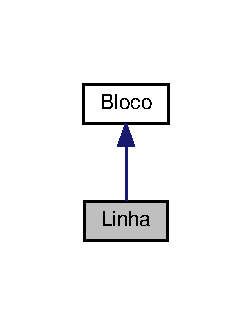
\includegraphics[width=121pt]{structLinha__inherit__graph}
\end{center}
\end{figure}


Diagrama de colaboração para Linha\+:\nopagebreak
\begin{figure}[H]
\begin{center}
\leavevmode
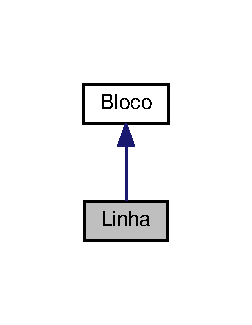
\includegraphics[width=121pt]{structLinha__coll__graph}
\end{center}
\end{figure}
\subsection*{Métodos Públicos}
\begin{DoxyCompactItemize}
\item 
\hyperlink{structLinha_a4482bff9f7dc3c59b801b88c9b524f70}{Linha} (unsigned int tamanho)
\begin{DoxyCompactList}\small\item\em Cria uma \hyperlink{structLinha}{Linha} (\hyperlink{structBloco}{Bloco}) de \{tamanho\} palavras. \end{DoxyCompactList}\item 
\hyperlink{structLinha}{Linha} \& \hyperlink{structLinha_a93ee2fba6780638546c4bbf78445e8bc}{ler} (\hyperlink{structBloco}{Bloco} \&bloco, unsigned int \hyperlink{structLinha_ab9ce9d1248c2abd2211539f09d8c6e0a}{numero\+\_\+do\+\_\+bloco}, unsigned int tamanho\+\_\+do\+\_\+conjunto, unsigned int acessos)
\begin{DoxyCompactList}\small\item\em lê um bloco da mémoria (armazena na linha). \end{DoxyCompactList}\item 
\hyperlink{structLinha}{Linha} \& \hyperlink{structLinha_aa7aa98581c6cd16951abb275fe78727d}{escrever} (unsigned int palavra, unsigned int valor)
\begin{DoxyCompactList}\small\item\em escreve uma valor dentro do vetor de palavras. \end{DoxyCompactList}\item 
bool \hyperlink{structLinha_a7c1d9293e17a1919e53dc35df4c2e5c3}{buscar} (unsigned int \hyperlink{structLinha_ab9ce9d1248c2abd2211539f09d8c6e0a}{numero\+\_\+do\+\_\+bloco}, unsigned int acessos)
\begin{DoxyCompactList}\small\item\em Verifica se o bloco está nessa linha. \end{DoxyCompactList}\end{DoxyCompactItemize}
\subsection*{Atributos Públicos}
\begin{DoxyCompactItemize}
\item 
\mbox{\Hypertarget{structLinha_ab9ce9d1248c2abd2211539f09d8c6e0a}\label{structLinha_ab9ce9d1248c2abd2211539f09d8c6e0a}} 
unsigned int \hyperlink{structLinha_ab9ce9d1248c2abd2211539f09d8c6e0a}{numero\+\_\+do\+\_\+bloco}
\begin{DoxyCompactList}\small\item\em Cada linha tem o número do bloco que está armazenado. \end{DoxyCompactList}\item 
\mbox{\Hypertarget{structLinha_acb0cf5d63a5ae6a9fd604ef302c053b8}\label{structLinha_acb0cf5d63a5ae6a9fd604ef302c053b8}} 
unsigned int \hyperlink{structLinha_acb0cf5d63a5ae6a9fd604ef302c053b8}{total\+\_\+de\+\_\+usos}
\begin{DoxyCompactList}\small\item\em contador usado no L\+FU. \end{DoxyCompactList}\item 
\mbox{\Hypertarget{structLinha_a645231426689a6887121c3fc916c3bc1}\label{structLinha_a645231426689a6887121c3fc916c3bc1}} 
unsigned int \hyperlink{structLinha_a645231426689a6887121c3fc916c3bc1}{refencia\+\_\+temporal}
\begin{DoxyCompactList}\small\item\em contador usado no L\+RU. \end{DoxyCompactList}\item 
\mbox{\Hypertarget{structLinha_ad08975892e9a9d9a4b2902fbfc7426a3}\label{structLinha_ad08975892e9a9d9a4b2902fbfc7426a3}} 
unsigned int \hyperlink{structLinha_ad08975892e9a9d9a4b2902fbfc7426a3}{chegada}
\begin{DoxyCompactList}\small\item\em contador usado no F\+I\+FO. \end{DoxyCompactList}\end{DoxyCompactItemize}


\subsection{Descrição Detalhada}
A linha é um bloco da cache, com a diferença que ela contém os contadores. 

\subsection{Construtores \& Destrutores}
\mbox{\Hypertarget{structLinha_a4482bff9f7dc3c59b801b88c9b524f70}\label{structLinha_a4482bff9f7dc3c59b801b88c9b524f70}} 
\index{Linha@{Linha}!Linha@{Linha}}
\index{Linha@{Linha}!Linha@{Linha}}
\subsubsection{\texorpdfstring{Linha()}{Linha()}}
{\footnotesize\ttfamily Linha\+::\+Linha (\begin{DoxyParamCaption}\item[{unsigned int}]{tamanho }\end{DoxyParamCaption})\hspace{0.3cm}{\ttfamily [inline]}}



Cria uma \hyperlink{structLinha}{Linha} (\hyperlink{structBloco}{Bloco}) de \{tamanho\} palavras. 


\begin{DoxyParams}{Parâmetros}
{\em tamanho} & quantidade de palavras. \\
\hline
\end{DoxyParams}


\subsection{Métodos}
\mbox{\Hypertarget{structLinha_a7c1d9293e17a1919e53dc35df4c2e5c3}\label{structLinha_a7c1d9293e17a1919e53dc35df4c2e5c3}} 
\index{Linha@{Linha}!buscar@{buscar}}
\index{buscar@{buscar}!Linha@{Linha}}
\subsubsection{\texorpdfstring{buscar()}{buscar()}}
{\footnotesize\ttfamily bool Linha\+::buscar (\begin{DoxyParamCaption}\item[{unsigned int}]{numero\+\_\+do\+\_\+bloco,  }\item[{unsigned int}]{acessos }\end{DoxyParamCaption})\hspace{0.3cm}{\ttfamily [inline]}}



Verifica se o bloco está nessa linha. 


\begin{DoxyParams}{Parâmetros}
{\em numero\+\_\+do\+\_\+bloco} & numero do bloco na mémoria. \\
\hline
{\em acessos} & quantidade de acessos (usada como referência temporal para o L\+RU). \\
\hline
\end{DoxyParams}
\begin{DoxyReturn}{Retorna}
true, em caso de cache hit, false caso o contrário. 
\end{DoxyReturn}
\begin{DoxyNote}{Observação}
Os contadores de uso e referência temporal são atualizados aqui. 
\end{DoxyNote}
\mbox{\Hypertarget{structLinha_aa7aa98581c6cd16951abb275fe78727d}\label{structLinha_aa7aa98581c6cd16951abb275fe78727d}} 
\index{Linha@{Linha}!escrever@{escrever}}
\index{escrever@{escrever}!Linha@{Linha}}
\subsubsection{\texorpdfstring{escrever()}{escrever()}}
{\footnotesize\ttfamily \hyperlink{structLinha}{Linha}\& Linha\+::escrever (\begin{DoxyParamCaption}\item[{unsigned int}]{palavra,  }\item[{unsigned int}]{valor }\end{DoxyParamCaption})\hspace{0.3cm}{\ttfamily [inline]}}



escreve uma valor dentro do vetor de palavras. 


\begin{DoxyParams}{Parâmetros}
{\em palavra} & índice da palavra (endereço da palavra -\/ endereço da primeira palavra do conjunto). \\
\hline
{\em valor} & valor a ser colocado. \\
\hline
\end{DoxyParams}
\begin{DoxyReturn}{Retorna}
a própria linha. 
\end{DoxyReturn}
\mbox{\Hypertarget{structLinha_a93ee2fba6780638546c4bbf78445e8bc}\label{structLinha_a93ee2fba6780638546c4bbf78445e8bc}} 
\index{Linha@{Linha}!ler@{ler}}
\index{ler@{ler}!Linha@{Linha}}
\subsubsection{\texorpdfstring{ler()}{ler()}}
{\footnotesize\ttfamily \hyperlink{structLinha}{Linha}\& Linha\+::ler (\begin{DoxyParamCaption}\item[{\hyperlink{structBloco}{Bloco} \&}]{bloco,  }\item[{unsigned int}]{numero\+\_\+do\+\_\+bloco,  }\item[{unsigned int}]{tamanho\+\_\+do\+\_\+conjunto,  }\item[{unsigned int}]{acessos }\end{DoxyParamCaption})\hspace{0.3cm}{\ttfamily [inline]}}



lê um bloco da mémoria (armazena na linha). 


\begin{DoxyParams}{Parâmetros}
{\em bloco} & bloco da mémoria. \\
\hline
{\em numero\+\_\+do\+\_\+bloco} & Número do bloco dentro da mémoria principal. \\
\hline
{\em tamanho\+\_\+do\+\_\+conjunto} & tamanho do conjunto usado no mapeamento. \\
\hline
{\em acessos} & A quantidade de acessos é usada como referência temporal. \\
\hline
\end{DoxyParams}
\begin{DoxyReturn}{Retorna}
a própria linha. 
\end{DoxyReturn}
\begin{DoxyNote}{Observação}
os contadores são inicializados aqui. 
\end{DoxyNote}


A documentação para esta estrutura foi gerada a partir do seguinte arquivo\+:\begin{DoxyCompactItemize}
\item 
include/cache.\+hpp\end{DoxyCompactItemize}

\hypertarget{structMemoria}{}\section{Referência da Estrutura Memoria}
\label{structMemoria}\index{Memoria@{Memoria}}


A mémoria é um conjunto de blocos.  




{\ttfamily \#include $<$cache.\+hpp$>$}

\subsection*{Métodos Públicos}
\begin{DoxyCompactItemize}
\item 
\hyperlink{structMemoria_aacd10b6010e4839a83a260a59996161c}{Memoria} (unsigned int tamanho, unsigned int numero\+\_\+de\+\_\+palavras)
\begin{DoxyCompactList}\small\item\em Constrói uma memoria de \{tamanho\} blocos com cada bloco contendo \{numero\+\_\+de\+\_\+palavras\} palavras. \end{DoxyCompactList}\end{DoxyCompactItemize}
\subsection*{Atributos Públicos}
\begin{DoxyCompactItemize}
\item 
\mbox{\Hypertarget{structMemoria_a63701165b1d3d472685c47a7c2ad35ff}\label{structMemoria_a63701165b1d3d472685c47a7c2ad35ff}} 
std\+::vector$<$ \hyperlink{structBloco}{Bloco} $>$ \hyperlink{structMemoria_a63701165b1d3d472685c47a7c2ad35ff}{blocos}
\begin{DoxyCompactList}\small\item\em Vetor de blocos. \end{DoxyCompactList}\end{DoxyCompactItemize}


\subsection{Descrição Detalhada}
A mémoria é um conjunto de blocos. 

\subsection{Construtores \& Destrutores}
\mbox{\Hypertarget{structMemoria_aacd10b6010e4839a83a260a59996161c}\label{structMemoria_aacd10b6010e4839a83a260a59996161c}} 
\index{Memoria@{Memoria}!Memoria@{Memoria}}
\index{Memoria@{Memoria}!Memoria@{Memoria}}
\subsubsection{\texorpdfstring{Memoria()}{Memoria()}}
{\footnotesize\ttfamily Memoria\+::\+Memoria (\begin{DoxyParamCaption}\item[{unsigned int}]{tamanho,  }\item[{unsigned int}]{numero\+\_\+de\+\_\+palavras }\end{DoxyParamCaption})\hspace{0.3cm}{\ttfamily [inline]}}



Constrói uma memoria de \{tamanho\} blocos com cada bloco contendo \{numero\+\_\+de\+\_\+palavras\} palavras. 


\begin{DoxyParams}{Parâmetros}
{\em tamanho} & numero de blocos (definido na configuração).. \\
\hline
{\em numero\+\_\+de\+\_\+palavras} & número de palavras de cada bloco (definido na configuração).. \\
\hline
\end{DoxyParams}


A documentação para esta estrutura foi gerada a partir do seguinte arquivo\+:\begin{DoxyCompactItemize}
\item 
include/cache.\+hpp\end{DoxyCompactItemize}

\hypertarget{structRandom}{}\section{Referência da Estrutura Random}
\label{structRandom}\index{Random@{Random}}


Functor (objeto de função) para gerar números aléatorios não negativos de três digitos.  




{\ttfamily \#include $<$cache.\+hpp$>$}

\subsection*{Métodos Públicos}
\begin{DoxyCompactItemize}
\item 
\mbox{\Hypertarget{structRandom_adcf65dea31f990d9d7ec536fed7aa6ca}\label{structRandom_adcf65dea31f990d9d7ec536fed7aa6ca}} 
int {\bfseries operator()} ()
\end{DoxyCompactItemize}
\subsection*{Atributos Públicos}
\begin{DoxyCompactItemize}
\item 
\mbox{\Hypertarget{structRandom_a7206399225b174d8a582fbe005fdd147}\label{structRandom_a7206399225b174d8a582fbe005fdd147}} 
std\+::random\+\_\+device {\bfseries rd}
\item 
\mbox{\Hypertarget{structRandom_aa4354db31fa7d64040939b905ab12ee1}\label{structRandom_aa4354db31fa7d64040939b905ab12ee1}} 
std\+::mt19937 {\bfseries mt}
\item 
\mbox{\Hypertarget{structRandom_a526c9d413a18965b3075bfcc23c28dcb}\label{structRandom_a526c9d413a18965b3075bfcc23c28dcb}} 
std\+::uniform\+\_\+int\+\_\+distribution$<$ unsigned int $>$ {\bfseries dist}
\end{DoxyCompactItemize}


\subsection{Descrição Detalhada}
Functor (objeto de função) para gerar números aléatorios não negativos de três digitos. 

A documentação para esta estrutura foi gerada a partir do seguinte arquivo\+:\begin{DoxyCompactItemize}
\item 
include/cache.\+hpp\end{DoxyCompactItemize}

%--- End generated contents ---

% Index
\backmatter
\newpage
\phantomsection
\clearemptydoublepage
\addcontentsline{toc}{chapter}{Índice}
\printindex

\end{document}
